\subsection{交易闭环搜索问题}
具体问题描述可见 \ref{pro1} 交易闭环搜索问题 一节.

此问题涉及的数据文件有:
\begin{itemize}
  \item Account.csv(点)
  \item AccountTransferAccount.csv(边)
\end{itemize}

\subsubsection{输入}
\begin{center}
\begin{minted}[xleftmargin=5mm]{java}
// 构建点
PWindowSource<IVertex<String, Integer>> vertices = pipelineTaskCxt
  .buildSource(
    new FileSource<IVertex<String, Integer>>(
      "Account.csv",
      line -> {
        String[] fields = line.split("\\|");
        // <vertexKey, vertexValue>: <String, Integer>
        // 此处以 Account 的 Id 作为点的 Id,
        // 点的值为以此点为源点的三角形的个数
        IVertex<String, Integer> vertex = new ValueVertex<String, Integer>(
        fields[0], 0);
        return Collections.singletonList(vertex);
    }),
    AllWindow.getInstance())
  .withParallelism(sourceParallelism);

// 构建边
PWindowSource<IEdge<String, String>> edges = pipelineTaskCxt
  .buildSource(
    new FileSource<IEdge<String, String>>(
      "AccountTransferAccount.csv",
      line -> {
        String[] fields = line.split("\\|");
        // <vertexKey, edgeValue>: <String, String>
        // 此处以 Account 的 Id 作为点的 Id
        IEdge<String, String> edge = new ValueEdge<String, String>(
          fields[0], fields[1], ""); // (srcId, targetId, edgeValue)
        return Collections.singletonList(edge);
    }),
    AllWindow.getInstance())
  .withParallelism(sourceParallelism);

// 构造图视图(用于将构造出的点和边关联起来)
GraphViewDesc graphViewDesc = GraphViewBuilder
  .createGraphView(GraphViewBuilder.DEFAULT_GRAPH)
  .withShardNum(iterationParallelism)
  .withBackend(BackendType.Memory)
  .build();
\end{minted}
\end{center}

\subsubsection{核心算法}
此问题可看作是寻找图中三角形 $ K^{3} $ 的个数.

对图中的某个点 $ A $, $ A $ 向每个相邻点发送消息 $ M=(1, A) $, 此后消息
$ M $ 每传递一次, $ M $ 的第一个元素的值就增加 $ 1 $, 若 $ A $ 在某个三角形中,
则 $ M $ 最终会被传回给 $ A $, 此时 $ M = (3, A) $, 点 $ A $
发现这是自己发出的消息, 于是更新状态(以 $ A $ 为源点的三角形个数);
若 $ M $ 的第一个元素的值为 $ 3 $ 且消息到达的点的 Id 与 $ M $ 的第二个元素不等,
则丢弃该消息, 不再继续传递.

\begin{figure}[H]
  \begin{center}
    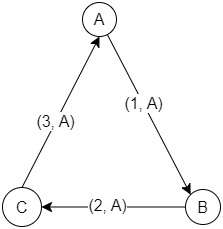
\includegraphics[width=0.15\textwidth]{./figures/pro1.jpg}
  \end{center}
  \caption{交易闭环搜索消息传递}
\end{figure}

\begin{center}
\begin{minted}[xleftmargin=5mm]{java}
public void compute(
  String vertexId, Iterator<String> messageIterator) {
  IVertex<String, Integer> vertex = this.context.vertex().get();

  // 首轮迭代向所有相邻节点发送消息
  if (this.context.getIterationId() == 1L) {
    this.context.sendMessageToNeighbors("1," + vertexId);
  }

  while (messageIterator.hasNext()) {
    String[] msg = messageIterator.next().split(",");
    int t = Integer.parseInt(msg[0]);
    String msgId = msg[1];

    if (t < 3) {
      t += 1;
      if (t == 3) {
        List<IEdge<String, String>> edges = this.context
          .edges().getOutEdges();
        for (IEdge<String, String> edge : edges) {
          if (msgId.equals(edge.getTargetId())) {
            // 仅向可以形成闭环的点发送消息,
            // 避免非必要的内存浪费和减少计算的时间开销
            this.context.sendMessage(msgId, "3," + msgId);
          }
        }
      } else {
        this.context.sendMessageToNeighbors(
          Integer.toString(t) + "," + msgId);
      }
    } else if (t == 3) { // 找到一个闭环, 更新结果
      this.context.setNewVertexValue(vertex.getValue() + 1);
    }
  }
}
\end{minted}
\end{center}

\subsubsection{输出}
\begin{center}
\begin{minted}[xleftmargin=5mm]{java}
PWindowStream<IVertex<String, Integer>> result = pipelineTaskCxt
  .buildWindowStreamGraph(vertices, edges, graphViewDesc)
  .compute(new Case2Algorithms(4)) // 迭代 4 轮
  .compute(iterationParallelism)
  .getVertices();

SinkFunction<String> sink = ExampleSinkFunctionFactory
  .getSinkFunction(conf);
result
  .filter(v -> v.getValue() >= 1) // 过滤出符合要求的点
  .map(v -> String.format("%s|%s", v.getId(), v.getValue()))
  .withParallelism(mapParallelism)
  .sink(sink) // 写入文件
  .withParallelism(sinkParallelism);
\end{minted}
\end{center}
